\include{template}
\usepackage{mhchem}


%%%%%%%%%%%%%%%%%%%%%%%%%%%%%%%%%%%%%%%%%%%%%%%%%%%%%%%%%%%%%%%%%%%%%%%%%%%%%%%%%%%%%%
 
\title{\usebeamerfont*{title} Identification of cell signaling pathways 
    based on \\biochemical reaction kinetics repositories
}

\author{\vspace*{.5cm} \usebeamerfont*{author font} Gustavo Estrela de 
    Matos$^{\text{a, b, c}}$ \\ 
    \vspace*{.5cm}{\usebeamerfont*{supervisor font} Hugo Armelin$^{\text{b, c}}$, Marcelo S. Reis$^{\text{b, c}}$}}

\institute{%
    $^{\text{a}}$Institute of Mathematics and Statistics, University of São Paulo, Brazil\\%
$^{\text{b}}$Center of Toxins, Immune-response and Cell Signaling (CeTICS), Instituto Butantan, Brazil\\%
$^{\text{c}}$Special Laboratory of Cell Cycle, Instituto Butantan, Brazil}


\setbeamercolor{alerted text}{fg=alert_blue}

%%%%%%%%%%%%%%%%%%%%%%%%%%%%%%%%%%%%%%%%%%%%%%%%%%%%%%%%%%%%%%%%%%%%%%%%%%%%%%%%%%%%%%
\begin{document}


\renewcommand{\figurename}{Fig.}

\begin{frame}
\begin{columns}

\leftcolumn{ 
\begin{block}{Cell Signaling Pathways}%
\paragraph{
    Cell Signaling is a mechanism that allows the cell to change its 
    behaviour according to the environment.
\begin{figure}
    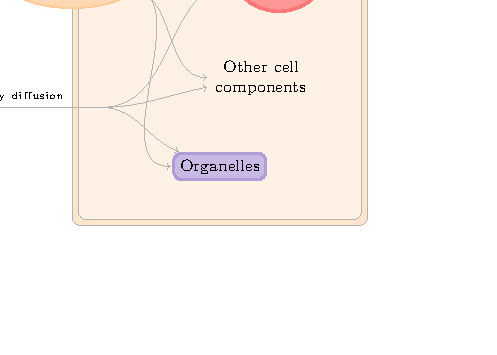
\includegraphics[width=.7\textwidth]{csp/signaling_mechanism.pdf}
\end{figure}
    A signal flows in a cell thorugh a cell signaling pathway, which can
    be characterized by a \alert{sequence of chemical reactions}.
}
\leftfigparagraph{csp/western_blot.png}{15}{6}{
    \hspace{1em}\\
    We can summarize the state of a \\
    cell signaling pathway by measuring \\
    the concentration over time of some \\ 
    chemical species that are present on \\
    the pathway.
}
\end{block}

%%%%%%%%%%%%%%%%%%%%%%%%%%%%%%%%%%%%%%%%%%%%%%%%%%%%%%%%%%%%%%%%%%%%%%%%                                     
\begin{block}{Identification of Signaling Pathways}%
\paragraph{
    What is the structure of a cell signaling pathway, given a set of 
    concentration measurements? We answer this question
    with a computational model, created from \alert{a set of chemical 
    reactions}, that can reproduce the concentration dynamics observed 
    experimentally. These models are created using the laws of 
    biochemical kinetics, deriving a system of ordinary differential 
    equations.
    
    %\begin{center}
    %\begin{tabular}{c c}
        %$\ce{
            %A + B -> C
        %}$ &  meu filhooo
    %\end{tabular}
    %\end{center}
    
        
}
\paragraph{
    As an example, we can model the following equation:
    \begin{equation*}
        \ce{A + B -> C} \implies \frac{d[C]}{dt} = k[A][B]
    \end{equation*}
    Where $k$ is a reaction rate constant.
}
\paragraph{
    However, to derive the model, we still need to determine what is
    the set of chemical reactions of the signaling pathway.
}
\end{block}

%\vspace{-1cm}
\begin{block}{Feature Selection}
\paragraph{
    We proposed to solve the identification of cell signaling pathways
    as a feature selection problem. This problem consists of: given 
    a set of features (reactions) and a score for each subset (the
    \alert{quality of a model}), what is the best subset?
    %\begin{figure}
        %\includegraphics[width=\textwidth]{featsel/featsel.pdf}
    %\end{figure}
}
\end{block}


\begin{block}{Bayesian Ranking of Models}
    To determine the \alert{quality of a model} we implemented a 
    score function that is a estimative of $p(D | M)$, which is the 
    likelihood of observing experiment $D$ under the assumption that 
    model $M$ is correct. To create this estimative we generate 
    samples of the posterior distribution of model 
    parameters ($\theta$).
    
    \begin{equation*}
        \underbrace{p (\theta | M, D)}_{\text{posterior}} \propto 
        \underbrace{p(D | M, \theta)}_{\text{likelihood}}
        \underbrace{p(\theta|M)}_{\text{prior}}
    \end{equation*}
    
    \leftfigparagraph{signetms_qr.png}{8}{4}{\hspace{1em}\\
        This ranking score was implemented as a Python package \\
        called SigNetMS. It is an open source software and \\
        it is available on GitHub.
    }
\end{block}

} % end \leftcolumn



%%%%%%%%%%%%%%%%%%%%%%%%%%%%%%%%%%%%%%%%%%%%%%%%%%%%%%%%%%%%%%%%%%%%%%%%
\rightcolumn{              
\begin{block}{The Proposed Methodology}%
    \begin{figure}
        \includegraphics[width=\textwidth]{featsel/featsel.pdf}
    \end{figure}
\end{block}


%%%%%%%%%%%%%%%%%%%%%%%%%%%%%%%%%%%%%%%%%%%%%%%%%%%%%%%%%%%%%%%%%%%
\begin{block}{Experiments}%
\paragraph{
}
\end{block}


%%%%%%%%%%%%%%%%%%%%%%%%%%%%%%%%%%%%%%%%%%%%%%%%%%%%%%%%%%%%%%%%%%%
\begin{block}{Conclusão}%
\paragraph{
}
\end{block}
%\vfill 
\vspace*{.5cm}%
\begin{block}{Acknowledgement}%
\vspace*{-1.5cm}%
\begin{figure}[h]
    \begin{tabular*}{0.7\textwidth}{c@{\extracolsep{\fill}}cc}
    \centering
    \subfigure {
        \includegraphics[clip=true, width=0.2\textwidth]{institutions/FAPESP.jpg}
    }
    &
    \subfigure {
        \includegraphics[clip=true, width=0.2\textwidth]{institutions/CNPq.png}
    }
    &
    \subfigure {
        \includegraphics[clip=true, width=0.1\textwidth]{institutions/capes.jpg}
    }
    \end{tabular*}   
\end{figure}
\vspace*{1.5cm}%
\end{block}%
}% end of right column
\end{columns}
\end{frame}
\end{document}
